\documentclass[11pt,psfig]{article}
\usepackage{epsfig}
\usepackage{times}
\usepackage{amssymb}
\usepackage{float}

\newcount\refno\refno=1
\def\ref{\the\refno \global\advance\refno by 1}
\def\ux{\underline{x}}
\def\uw{\underline{w}}
\def\bw{\underline{w}}
\def\ut{\underline{\theta}}
\def\umu{\underline{\mu}} 
\def\bmu{\underline{\mu}} 
\def\be{p_e^*}
\newcount\eqnumber\eqnumber=1
\def\eq{\the \eqnumber \global\advance\eqnumber by 1}
\def\eqs{\eq}
\def\eqn{\eqno(\eq)}

 \pagestyle{empty}
\def\baselinestretch{1.1}
\topmargin1in \headsep0.3in
\topmargin0in \oddsidemargin0in \textwidth6.5in \textheight8.5in
\begin{document}
\setlength{\parskip}{1.2ex plus0.3ex minus 0.3ex}


\thispagestyle{empty} \pagestyle{myheadings} \markright{Homework
\#: CS 216, Image Understanding: Spring 2014}



\title{CS 216 Homework 2}
\author{Zachary DeStefano, 15247592}
\date{Due Date: April 25, 2014}

\maketitle

\vfill\eject

\newpage

\section*{Problem 1}

We will prove that $(f*g)*h=f*(g*h)$. First off, let $x=f*g$ and let $y=g*h$. \\
\[
x(t) = (f*g)(t) = \sum_{s=-\infty}^{\infty} f(t-s)g(s)
\]
\[
y(t) = (g*h)(t) = \sum_{s=-\infty}^{\infty} g(s)h(t-s)
\]
This means that
\[
(x*h)(t) = \sum_{v=-\infty}^{\infty} x(v)h(t-v) = \sum_{v=-\infty}^{\infty} \sum_{s=-\infty}^{\infty} f(v-s)g(s)h(t-v)
\]
Similarly
\[
(f*y)(t) = \sum_{v=-\infty}^{\infty} f(t-v)y(v) = \sum_{v=-\infty}^{\infty} \sum_{s=-\infty}^{\infty} f(t-v)g(s)h(v-s)
\]
In the second equation, do a change of variables $v = t-v'+s$ which does not change the final result since we are going from negative infinity to infinity. For the second equation, we end up with \\
\[
(f*y)(t) = \sum_{v'=-\infty}^{\infty} \sum_{s=-\infty}^{\infty} f(v'-s)g(s)h(t-v')
\]
As can be observed, the first and second equation are now equal. This proves that $(x*h)(t)=(f*y)(t)$ and since this applies for any three functions, we have proven that convolution is associative. 

\newpage

\section*{Problem 2}

If we correlate a function $f$ with an impulse function, we get $f(-t)$, \\
so the function gets flipped around the y-axis. \\
Here is the proof:\\
Take the impulse function g, so $g(0)=1$ and $g(x)=0$ for all other $x$ \\
Let * be the correlation operation in this case. \\
\[
(f*g)(t) = \sum_{s=-\infty}^{\infty} f(s)g(s+t)
\]
In our case, the inner term is always $0$ except for when $s+t=0$ so $s=-t$, \\
thus $(f*g)(t)=f(-t)$, proving our assertion. \\
\\
Now let $h(t)=g(t)$. We will prove that $(f*g)*h \neq f*(g*h)$. \\
\\
For the right hand side, by what was shown above, \\
$g*h = g$ since the impulse function is symmetric around the y-axis. \\
This means that $(f*(g*h))(t) = (f*g)(t) = f(-t)$. \\
\\
For the left hand side, by what was shown above, \\
$(f*g)(t) = f(-t)$ thus $((f*g)*h)(t) = (f(-t))*h(t)$\\
This will flip the function back to its original position, thus the left hand side is equal to $f(t)$\\
\\
For any non-symmetric function $f$, such as $f(t) = 3t+5$, it holds that $f(t) \neq f(-t)$ \\
thus the left hand side is not equal to the right hand side. \\
\\
Since we have example functions whose correlations are not associative, there is no way correlation is associative. 

\newpage

\section*{Problem 3}

Let $g_1(x) = g_2(y) = N(0,\sigma^2)$. Then
\[
g_1(x) = \frac{1}{\sqrt{2\pi \sigma^2}} e^{-\frac{x^2}{2\sigma^2}}
\]
\[
g_2(y) = \frac{1}{\sqrt{2\pi \sigma^2}} e^{-\frac{y^2}{2\sigma^2}}
\]
This means that
\[
g_1(x)g_2(y) = \frac{1}{2\pi \sigma^2} e^{-\frac{x^2 + y^2}{2\sigma^2}}
\]
This is equal to $g(x,y)$, thus allowing us to say that $g(x,y) = g_1(x)g_2(y)$

\newpage

\section*{Problem 4}

For the spatial domain running time, we can think of convolution as the following:\\
- For each pixel in the image, we apply the filter to it. \\
Thus there are $H \cdot W$ iterations of the filter\\
Each filter will take $M \cdot N$ time. \\
Thus the time complexity is $O(MNHW)$\\
\\
If we use FFT, this would be the procedure:\\
1. Convert the signal to frequency\\
2. Convert the filter to frequency \\
3. Do element wise multiplication of the two new vectors. \\
4. Convert the elements back. \\
\\
Step 1 will take $MN \cdot log(MN)$ time\\
Step 2 will take $HW \cdot log(HW)$ time\\
Step 3 will take $max(HW,MN)$ time. The identity of the max will not matter in the end since the previous step eclipses this one. \\
Step 4 will take $max(HW,MN) log( max(HW, MN) )$ time. Again which one is the max does not matter because of step 1 and 2. \\
\\
The total running time is thus $O(MN \cdot log(MN) + HW \cdot log(HW) )$ in the case where we use FFT. \\
Assuming that $HW$ is the max, the running time is $O(HW \cdot log(HW))$. \\
\\
If the filter is $f(x,y) = f_1(x)f_2(y)$, let F be the Fourier transform, then the following happens by properties of convolution and the Fourier transform\\
\[
F( I*f ) = F(I) \cdot F(f) = F(I) \cdot (F(f_1) * F(f_2))
\]
Thus the procedure would be the following:\\
1. Compute FFT of horizontal filter\\
2. Compute FFT of the vertical filter\\
3. Do convolution of the two FFTs found\\
4. Compute FFT of the image\\
5. Do point-wise multiplication of the FFT of the image with the filter found in step 3. \\
\\
Step 1 and 2 will take $M log(M) + N log(N)$ time.  \\
Step 3 will take $MN$ time using the normal convolution procedure. \\
Step 4 will take $HW \cdot log(HW)$ time. \\
Assuming $HW$ dominates, step 5 will take $HW$ time. \\
Assuming that $HW$ is greater than $M$ or $N$, step 4 and 5 dominate. \\
The total running time is thus $O( HW \cdot log(HW) )$ time. \\
TODO: Check this

\newpage

\section*{Problem 5}

Our two gaussians are as follows
\[
g_1(t) = \frac{1}{\sqrt{2\pi \sigma_1^2}} e^{-\frac{t^2}{2\sigma_1^2}}
\]
\[
g_2(t) = \frac{1}{\sqrt{2\pi \sigma_2^2}} e^{-\frac{t^2}{2\sigma_2^2}}
\]
The convolution formula we will use is the following
\[
g_3(t) = \int_{-\infty}^{\infty}{g_1(s)g_2(t-s) \, ds}
\]
Let $F_1$ be the Fourier transform for $g_1$ and $F_2$ be the transform for $g_2$.\\
\[
F_1(t) = \int_{-\infty}^{\infty}{g_1(s) e^{-2\pi i s t} \, ds}
\]
\[
F_2(t) = \int_{-\infty}^{\infty}{g_2(s) e^{-2\pi i s t} \, ds}
\]
Expanding we have
\[
F_1(t) = \frac{1}{\sqrt{2 \pi \sigma_1^2}} \int_{-\infty}^{\infty}{e^{-\frac{s^2}{2\sigma_1^2}} e^{-2\pi i s t} \, ds}
\]
\[
F_2(t) = \frac{1}{\sqrt{2 \pi \sigma_2^2}} \int_{-\infty}^{\infty}{e^{-\frac{s^2}{2\sigma_2^2}} e^{-2\pi i s t} \, ds}
\]
Expanding the imaginery exponent
\[
F_1(t) = \frac{1}{\sqrt{2 \pi \sigma_1^2}} \int_{-\infty}^{\infty}{e^{-\frac{s^2}{2\sigma_1^2}} (cos(2\pi s t) + i sin(2\pi s t)) \, ds}
\]
\[
F_2(t) = \frac{1}{\sqrt{2 \pi \sigma_2^2}} \int_{-\infty}^{\infty}{e^{-\frac{s^2}{2\sigma_2^2}} (cos(2\pi s t) + i sin(2\pi s t)) \, ds}
\]
Since the sine is an odd function, the integral of it will go to zero, thus we can simply the above equations
\[
F_1(t) = \frac{1}{\sqrt{2 \pi \sigma_1^2}} \int_{-\infty}^{\infty}{e^{-\frac{s^2}{2\sigma_1^2}} cos(2\pi s t) \, ds}
\]
\[
F_2(t) = \frac{1}{\sqrt{2 \pi \sigma_2^2}} \int_{-\infty}^{\infty}{e^{-\frac{s^2}{2\sigma_2^2}} cos(2\pi s t) \, ds}
\]
By what was asserted in Wolfram Alpha, on this web page:
\begin{verbatim}
http://mathworld.wolfram.com/FourierTransformGaussian.html
\end{verbatim}
\[
F_1(t) = \frac{1}{\sqrt{2 \pi \sigma_1^2}} \sqrt{2 \pi \sigma_1^2} e^{-2 \pi^2 t^2 \sigma_1^2}
\]
\[
F_2(t) = \frac{1}{\sqrt{2 \pi \sigma_2^2}} \sqrt{2 \pi \sigma_2^2} e^{-2 \pi^2 t^2 \sigma_2^2}
\]
Simplifying we have the following
\[
F_1(t) = e^{-2 \pi^2 t^2 \sigma_1^2}
\]
\[
F_2(t) = e^{-2 \pi^2 t^2 \sigma_2^2}
\]
Let $F=F_1 \cdot F_2$ then we have
\[
F(t) = e^{-2 \pi^2 t^2 (\sigma_1^2 + \sigma_2^2)}
\]
Let $\sigma = -2 \pi^2 (\sigma_1^2 + \sigma_2^2)$, then 
\[
F(t) = e^{\sigma t^2}
\]
We want the inverse transform of that function to get the finished function. 
\[
g_3(x) = \int_{-\infty}^{\infty} e^{2\pi i x t} F(t) dt
\]
\[
g_3(x) = \int_{-\infty}^{\infty} e^{2\pi i x t}e^{\sigma t^2} dt
\]
From what we did before (TODO: Add in more detail)
\[
g_3(x) = \int_{-\infty}^{\infty} cos(2 \pi x t)e^{\sigma t^2} dt
\]
By the same logic used above, we can say that
\[
g_3(x) = \sqrt{-\frac{\pi}{\sigma}} \, e^{\frac{\pi^2 x^2}{\sigma}}
\]
Expanding $\sigma$ and then simplifying, we have
\[
g_3(x) = \sqrt{\frac{1}{2\pi (\sigma_1^2 + \sigma_2^2)}} \, e^{-\frac{x^2}{2(\sigma_1^2 + \sigma_2^2)}}
\]
If we let $\sigma_3 = \sqrt{\sigma_1^2 + \sigma_2^2}$ then we have
\[
g_3(x) = \sqrt{\frac{1}{2\pi \sigma_3^2}} \, e^{-\frac{x^2}{2\sigma_3^2}}
\]
This is clearly a Gaussian, thus we have proved that $g_3$ is a Gaussian with the variance of $\sigma_3$ as defined above. 


\section*{Problem 6}

Here are the initial plots

\begin{figure}[H]
\centering
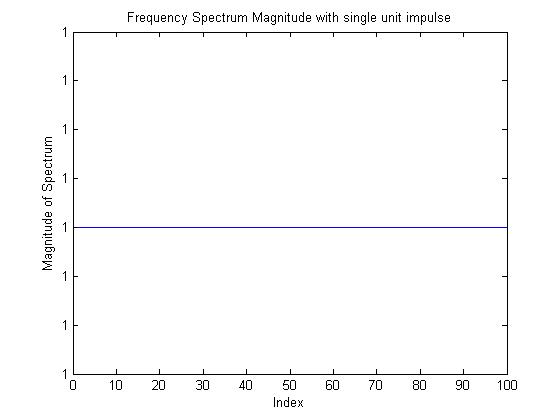
\includegraphics[height=3in]{prob6plot_freq1.jpg}
\caption{Frequency Spectrum Magnitude Plot for single impulse}
\end{figure}

\begin{figure}[H]
\centering
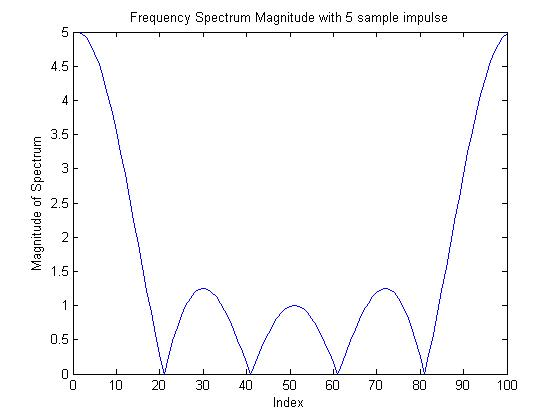
\includegraphics[height=3in]{prob6plot_freq5.jpg}
\caption{Frequency Spectrum Magnitude Plot for 5 sample impulse}
\end{figure}

\begin{figure}[H]
\centering
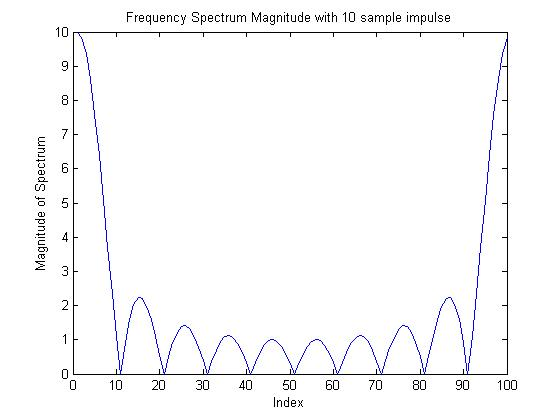
\includegraphics[height=3in]{prob6plot_freq10.jpg}
\caption{Frequency Spectrum Magnitude Plot for 10 sample impulse}
\end{figure}

\begin{figure}[H]
\centering
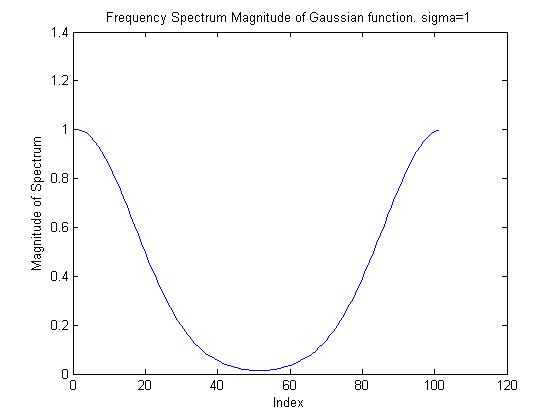
\includegraphics[height=3in]{prob6plot_freqGauss1.jpg}
\caption{Frequency Spectrum Magnitude Plot for Gaussian Function with $\sigma=1$}
\end{figure}

\begin{figure}[H]
\centering
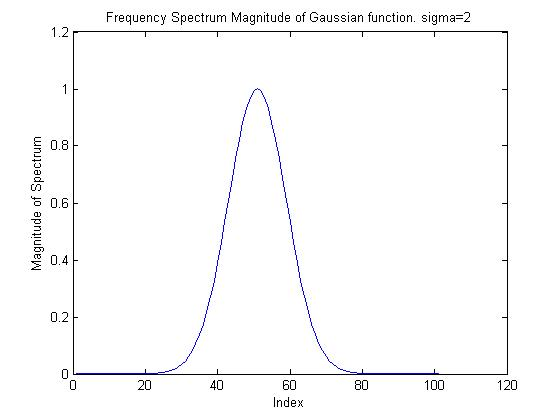
\includegraphics[height=3in]{prob6plot_freqGauss2.jpg}
\caption{Frequency Spectrum Magnitude Plot for Gaussian Function with $\sigma=2$}
\end{figure}

Here is the magnitude, phase experiment results

\begin{figure}[H]
\centering
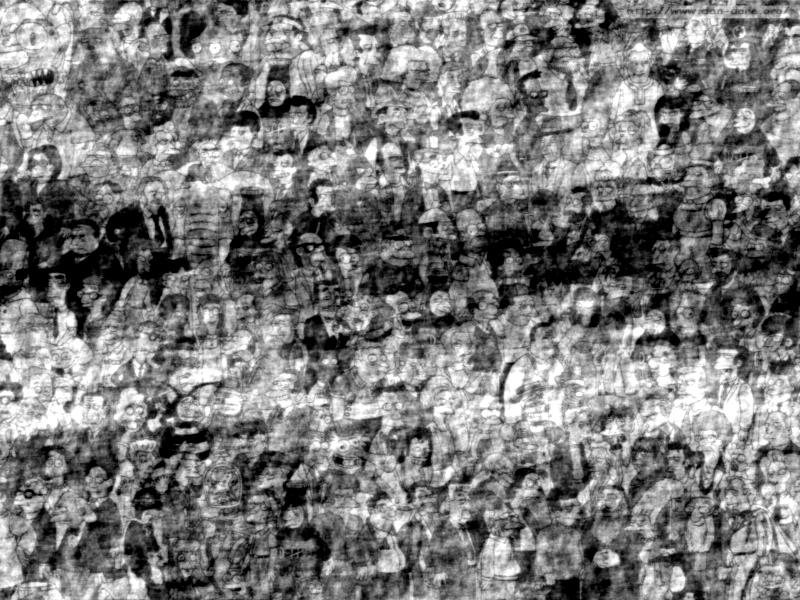
\includegraphics[height=3in]{mag_zebra_phase_simpsons.jpg}
\caption{Magnitude of Zebra picture with Phase of Simpsons picture}
\end{figure}

\section*{Problem 7}

Pictures for the Zebra image

\begin{figure}[H]
\centering
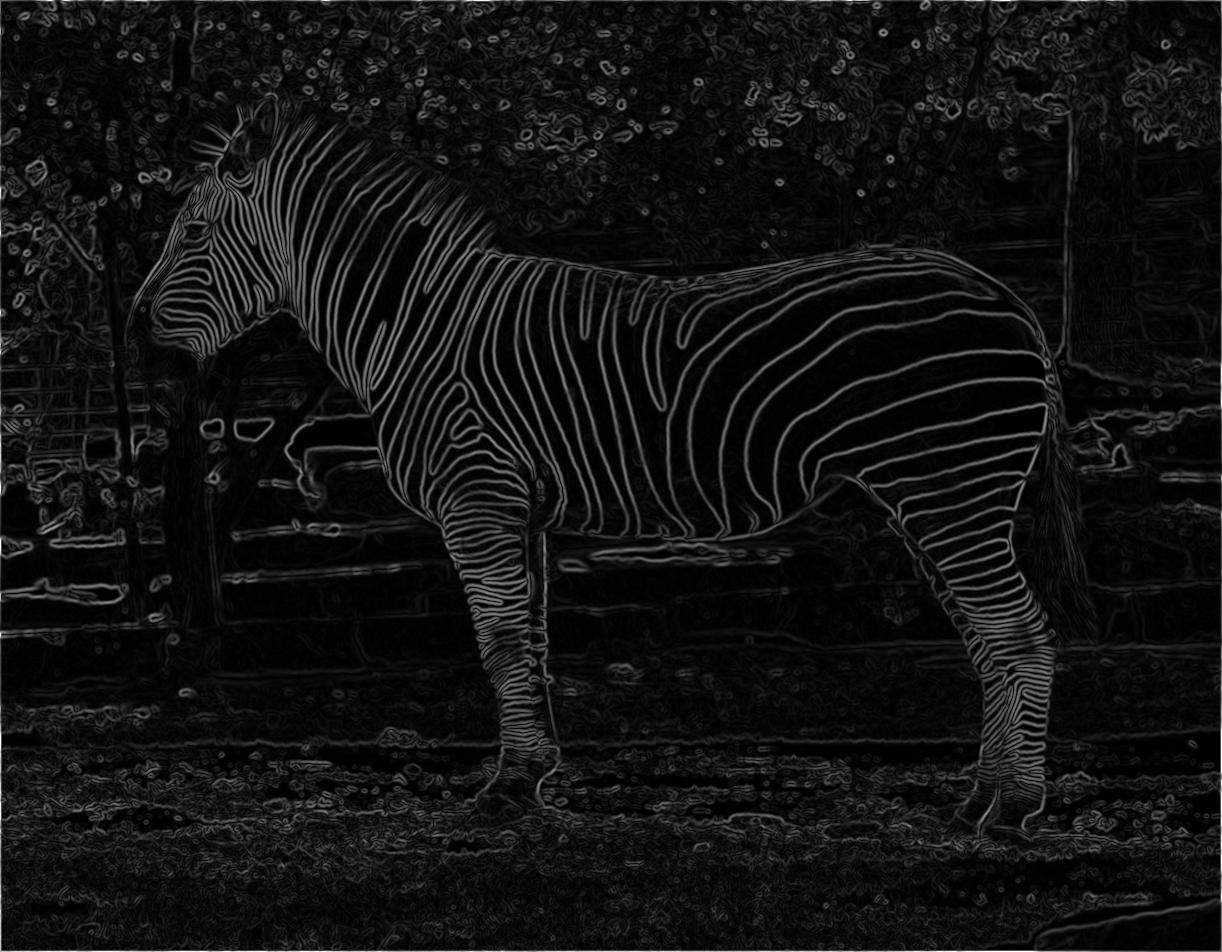
\includegraphics[height=3in]{magGradient_zebra1.jpg}
\caption{Magnitude of the Gradient of the zebra picture where $\sigma=3$}
\end{figure}

\begin{figure}[H]
\centering
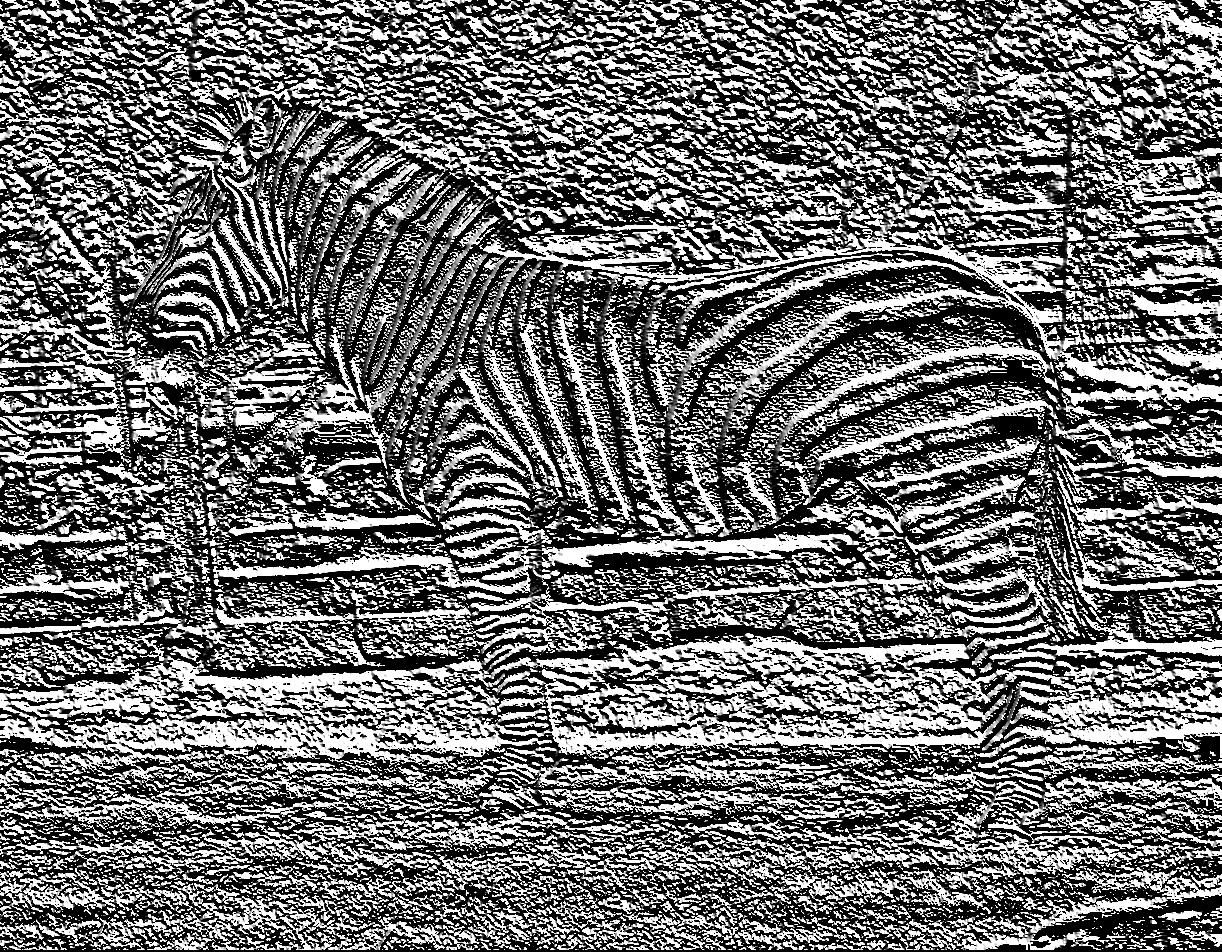
\includegraphics[height=3in]{orientGradient_zebra1.jpg}
\caption{Orientation of the Gradient of the zebra picture where $\sigma=3$}
\end{figure}

With new sigma

\begin{figure}[H]
\centering
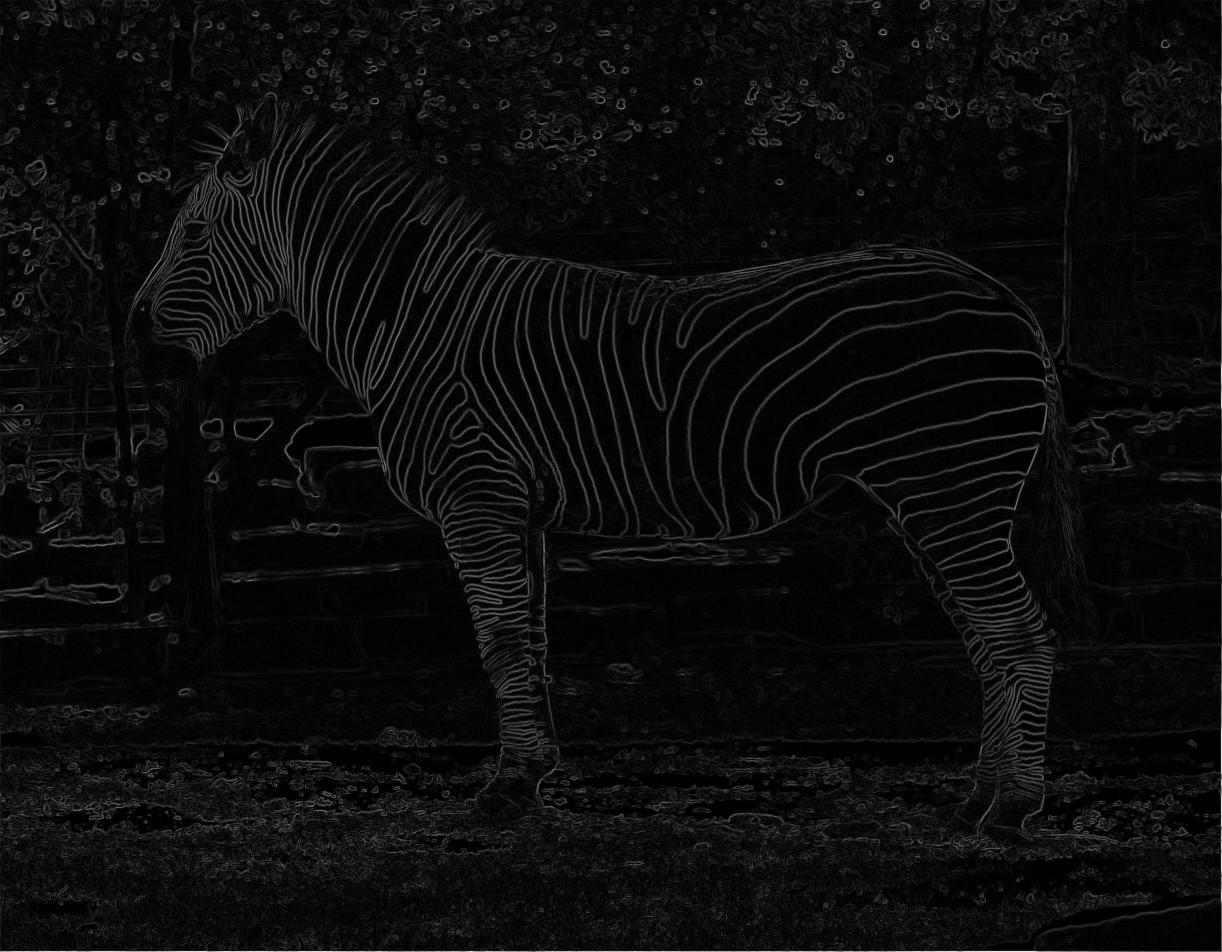
\includegraphics[height=3in]{magGradient2_zebra1.jpg}
\caption{Magnitude of the Gradient of the zebra picture where $\sigma=2$}
\end{figure}

\begin{figure}[H]
\centering
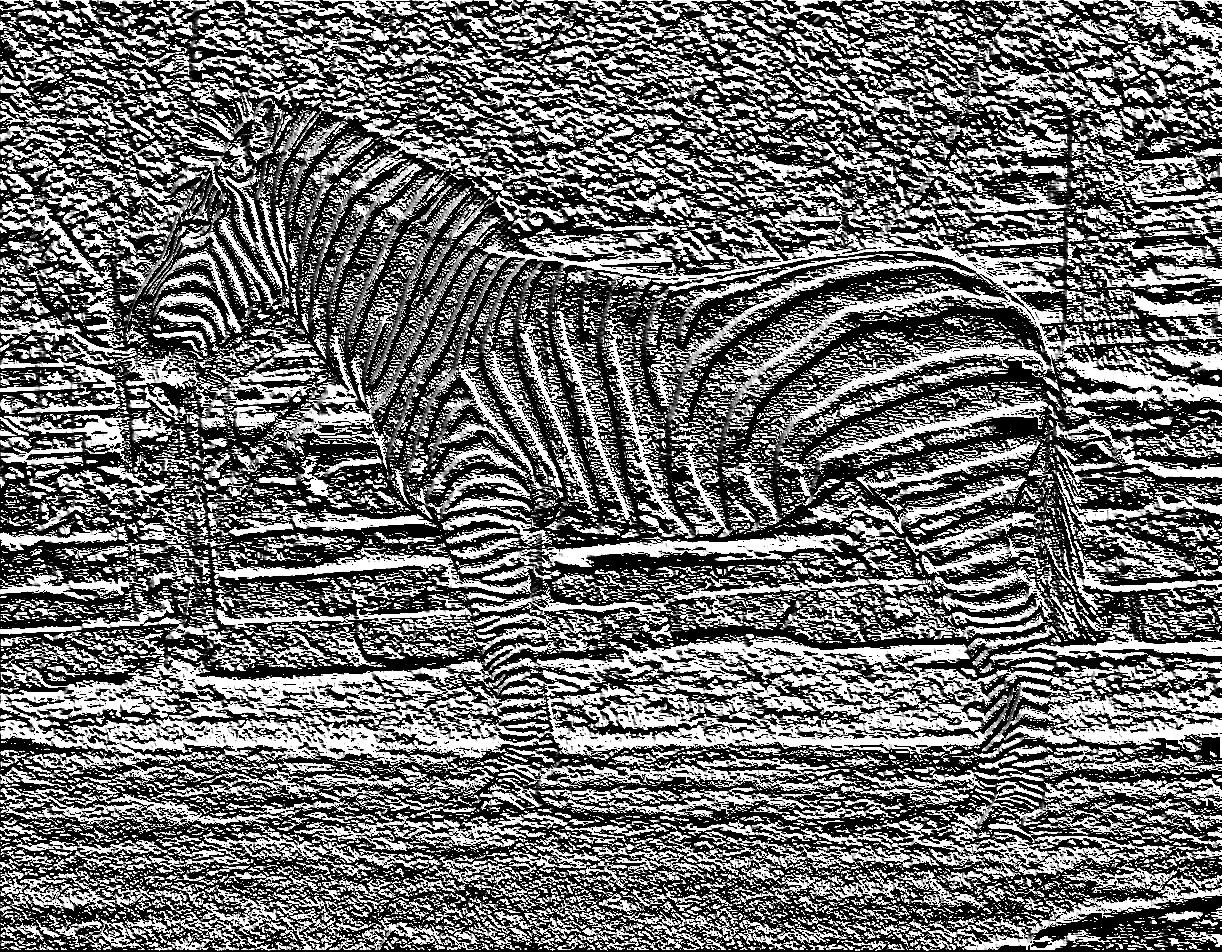
\includegraphics[height=3in]{orientGradient2_zebra1.jpg}
\caption{Orientation of the Gradient of the zebra picture where $\sigma=2$}
\end{figure}

\end{document}








